\documentclass[11pt]{article}
\usepackage[T1]{fontenc} % Use T1 font encoding
\usepackage[utf8]{inputenc} % Ensure UTF-8 encoding
\usepackage[polish]{babel} % Enable Polish language support
\usepackage{amsmath}
\usepackage{graphicx}
\usepackage{booktabs}
\usepackage{float}
\usepackage[margin=2.5cm]{geometry}
\usepackage{siunitx}
\usepackage{titlesec}
\titlespacing*{\subsection}{0pt}{*0.5}{*0.5} % Adjusts spacing before and after subsections
\usepackage{caption}
\usepackage{lmodern}
\usepackage{placeins} % For FloatBarrier
\usepackage{hyperref} % For hyperlinks in the document
\usepackage{threeparttable} % For better table handling
\usepackage{longtable} % For tables spanning multiple pages
\usepackage{fancyhdr} % For headers and footers
\usepackage{array} % For better table formatting
\usepackage{xcolor} % For colors

\title{Sprawozdanie z Laboratorium Fizyki: Termiczny Współczynnik oporu przewodnika}
\date{}

\begin{document}

% --------------------------- STRONA TYTUŁOWA --------------------------
\thispagestyle{empty} % Remove page number from title page

\begin{center}
    {\Large\textbf{UNIWERSYTET RADOMSKI}} \\
    \textit{im. Kazimierza Pułaskiego w Radomiu} \\
    \vspace{0.3cm}
    {\large\textbf{LABORATORIUM PODSTAW ELEKTRONIKI}} \\
\end{center}

\vspace{1.5cm}

% Main information box
\begin{center}
\fbox{\begin{minipage}{0.9\textwidth}
\centering
\vspace{0.5cm}
{\Large\textbf{SPRAWOZDANIE Z ĆWICZENIA}} \\
\vspace{0.8cm}
{\LARGE\textbf{Wzmacniacz}} \\
\vspace{0.5cm}
\end{minipage}}
\end{center}

\vspace{1.5cm}

% Information table
\begin{center}
\begin{tabular}{|>{\bfseries}p{4cm}|p{6cm}|}
\hline
Wydział: & WTEiI \\
\hline
Kierunek: & Informatyka \\
\hline
Rok Akademicki: & 2024/2025 \\
\hline
Semestr: & II \\
\hline
Grupa: & 3 \\
\hline
Zespół: & 2 \\
\hline
Wykonujący: & Jakub Oleszczuk \\
& Mateusz Ofiara \\
& Mikołaj Majewski \\
& Onolbataar Tumentur \\
\hline
Ocena: &  \\
\hline
\end{tabular}
\end{center}

\vspace{2cm}

% --------------------------- TREŚĆ SPRAWOZDANIA --------------------------
\subsection*{Cel ćwiczenia}
% Wzmacniacz byl badany bez C_E i bez R_0
% Wzmacniacz byl badany bez C_E z R_0
% Wzmacniacz byl badany z C_E i z R_0
% Wzmacniacz byl badany z C_E i bez R_0
% Konfiguracje

Celem ćwiczenia było zbadanie działania wzmacniacza operacyjnego w różnych konfiguracjach, 
a także analiza wpływu kondensatora i rezystora na charakterystykę wzmacniacza. W szczególności badano:
\begin{itemize}
    \item Wpływ kondensatora $C_E$ na stabilność i czas reakcji wzmacniacza.
    \item Wpływ rezystora $R_0$ na impedancję wejściową i wyjściową wzmacniacza.
    \item Porównanie charakterystyk wzmacniacza w różnych konfiguracjach (z $C_E$ i $R_0$, bez $C_E$ i $R_0$).
\end{itemize}

\clearpage
\section*{Wyniki pomiarów}
\subsection*{Tabela wyników}

% Tabele w układzie 2x2
\begin{figure}[!ht]
\centering

% Pierwszy rząd tabel
\begin{minipage}[t]{0.48\textwidth}
\centering
\captionof{table}{Konfiguracja bez kondensatora $C_E$ i rezystora $R_0$}
\begin{tabular}{|l|l|l|l|l|}
\hline
    f & U-we & U-wy & K & lg(f) \\ \hline
    2 & 0.5 & 0.04 & 0.08 & 0.301029996 \\ \hline
    3 & 0.5 & 0.136 & 0.272 & 0.477121255 \\ \hline
    5 & 0.5 & 0.376 & 0.752 & 0.698970004 \\ \hline
    10 & 0.5 & 0.936 & 1.872 & 1 \\ \hline
    100 & 0.5 & 1.84 & 3.68 & 2 \\ \hline
    500 & 0.5 & 1.72 & 3.44 & 2.698970004 \\ \hline
    1000 & 0.5 & 1.66 & 3.32 & 3 \\ \hline
    2000 & 0.5 & 1.46 & 2.92 & 3.301029996 \\ \hline
    3000 & 0.5 & 1.24 & 2.48 & 3.477121255 \\ \hline
    4000 & 0.5 & 1.04 & 2.08 & 3.602059991 \\ \hline       
    6000 & 0.5 & 0.76 & 1.52 & 3.77815125 \\ \hline
\end{tabular}
\end{minipage}
\hfill
\begin{minipage}[t]{0.48\textwidth}
\centering
\captionof{table}{Konfiguracja bez kondensatora $C_E$ z rezystorem $R_0$}
\begin{tabular}{|l|l|l|l|l|}
\hline
    f & U-we & U-wy & K & lg(f) \\ \hline
    2 & 0.5 & 0.032 & 0.064 & 0.301029996 \\ \hline
    3 & 0.5 & 0.008 & 0.016 & 0.477121255 \\ \hline
    5 & 0.5 & 0.1 & 0.2 & 0.698970004 \\ \hline
    10 & 0.5 & 0.388 & 0.776 & 1 \\ \hline
    100 & 0.5 & 0.904 & 1.808 & 2 \\ \hline
    500 & 0.5 & 0.84 & 1.68 & 2.698970004 \\ \hline
    1000 & 0.5 & 0.84 & 1.68 & 3 \\ \hline
    2000 & 0.5 & 0.8 & 1.6 & 3.301029996 \\ \hline
    3000 & 0.5 & 0.76 & 1.52 & 3.477121255 \\ \hline
    4000 & 0.5 & 0.68 & 1.36 & 3.602059991 \\ \hline
    6000 & 0.5 & 0.576 & 1.152 & 3.77815125 \\ \hline
\end{tabular}
\end{minipage}

\vspace{1em}

% Drugi rząd tabel
\begin{minipage}[t]{0.48\textwidth}
\centering
\captionof{table}{Konfiguracja z kondensatorem $C_E$ i rezystorem $R_0$}
\begin{tabular}{|l|l|l|l|l|}
\hline
    f & U-we & U-wy & K & lg(f) \\ \hline
    2 & 0.5 & 0.004 & 0.008 & 0.301029996 \\ \hline
    3 & 0.5 & 0.07 & 0.14 & 0.477121255 \\ \hline
    5 & 0.5 & 0.336 & 0.672 & 0.698970004 \\ \hline
    10 & 0.5 & 1.16 & 2.32 & 1 \\ \hline
    100 & 0.5 & 3.56 & 7.12 & 2 \\ \hline
    500 & 0.5 & 3.04 & 6.08 & 2.698970004 \\ \hline
    1000 & 0.5 & 3.36 & 6.72 & 3 \\ \hline
    2000 & 0.5 & 2.16 & 4.32 & 3.301029996 \\ \hline
    3000 & 0.5 & 1.56 & 3.12 & 3.477121255 \\ \hline
    4000 & 0.5 & 1.24 & 2.48 & 3.602059991 \\ \hline
    6000 & 0.5 & 0.9 & 1.8 & 3.77815125 \\ \hline
\end{tabular}
\end{minipage}
\hfill
\begin{minipage}[t]{0.48\textwidth}
\centering
\captionof{table}{Konfiguracja z kondensatorem $C_E$ i bez rezystora $R_0$}
\begin{tabular}{|l|l|l|l|l|}
\hline
    f & U-we & U-wy & K & lg(f) \\ \hline
    2 & 0.5 & 0.9 & 1.8 & 0.301029996 \\ \hline
    3 & 0.5 & 1.36 & 2.72 & 0.477121255 \\ \hline
    5 & 0.5 & 1.8 & 3.6 & 0.698970004 \\ \hline
    10 & 0.5 & 2.52 & 5.04 & 1 \\ \hline
    100 & 0.5 & 4.32 & 8.64 & 2 \\ \hline
    500 & 0.5 & 5.72 & 11.44 & 2.698970004 \\ \hline
    1000 & 0.5 & 7.04 & 14.08 & 3 \\ \hline
    2000 & 0.5 & 2.98 & 5.96 & 3.301029996 \\ \hline
    3000 & 0.5 & 1.16 & 2.32 & 3.477121255 \\ \hline
    4000 & 0.5 & 0.42 & 0.84 & 3.602059991 \\ \hline
    6000 & 0.5 & 0.148 & 0.296 & 3.77815125 \\ \hline
\end{tabular}
\end{minipage}

\end{figure}
\FloatBarrier % Ensures that all figures and tables are processed before continuing

\clearpage
\section*{Wykres}
%Jest jeden tylko wykres
\begin{figure}[H]
    \centering
    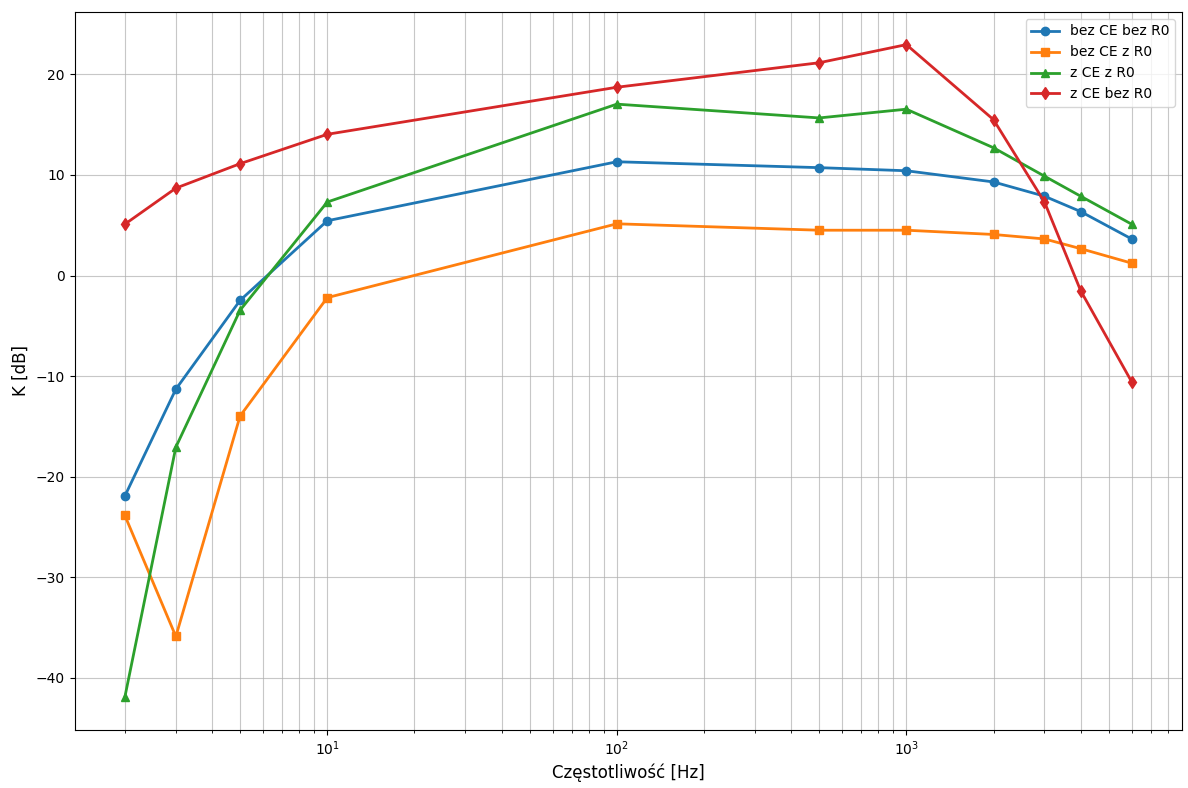
\includegraphics[width=0.8\textwidth]{wzmacniacz.png}
    \caption{Wykres zależności wzmocnienia od częstotliwości}
    \label{fig:wzmacniacz}
\end{figure}
\section*{Analiza wyników}
Wyniki pomiarów wykazały, że kondensator $C_E$ znacząco wpływa na charakterystykę wzmacniacza,
zwłaszcza w zakresie niskich częstotliwości, gdzie jego obecność zwiększa wzmocnienie.
Rezystor $R_0$ również ma istotny wpływ na impedancję wejściową i wyjściową wzmacniacza,
co może prowadzić do zmniejszenia wzmocnienia w przypadku jego obecności.
\section*{Wnioski}
Z przeprowadzonych badań wynika, że:
\begin{itemize}
    \item Kondensator $C_E$ poprawia stabilność wzmacniacza i zwiększa jego wzmocnienie w niskich częstotliwościach.
    \item Obecność rezystora $R_0$ wpływa na impedancję wzmacniacza, co może prowadzić do zmniejszenia wzmocnienia.
    \item Wzmacniacz operacyjny może być skutecznie używany w różnych konfiguracjach, w zależności od wymagań aplikacji.
    \item Analiza charakterystyki wzmacniacza w różnych konfiguracjach pozwala na lepsze zrozumienie jego działania i optymalizację parametrów dla konkretnych zastosowań.
\end{itemize}
\end{document}
